% This must be in the first 5 lines to tell arXiv to use pdfLaTeX, which is strongly recommended.
\pdfoutput=1
% In particular, the hyperref package requires pdfLaTeX in order to break URLs across lines.

\documentclass[11pt]{article}

% Remove the "review" option to generate the final version.
%\usepackage[review]{acl}
\usepackage[]{acl}

% Standard package includes
\usepackage{times}
\usepackage{latexsym}

% For proper rendering and hyphenation of words containing Latin characters (including in bib files)
\usepackage[T1]{fontenc}
% For Vietnamese characters
% \usepackage[T5]{fontenc}
% See https://www.latex-project.org/help/documentation/encguide.pdf for other character sets

% This assumes your files are encoded as UTF8
\usepackage[utf8]{inputenc}

% This is not strictly necessary, and may be commented out,
% but it will improve the layout of the manuscript,
% and will typically save some space.
\usepackage{microtype}

\usepackage[dvipsnames]{xcolor}
\newcommand{\AL}[1]{{\color{blue}{[Andrew: #1]}}}

% If the title and author information does not fit in the area allocated, uncomment the following
%
%\setlength\titlebox{<dim>}
%
% and set <dim> to something 5cm or larger.

\title{Unsupervised Lexical Semantic Change Detection via Influences Function}

% Author information can be set in various styles:
% For several authors from the same institution:
% \author{Author 1 \and ... \and Author n \\
%         Address line \\ ... \\ Address line}
% if the names do not fit well on one line use
%         Author 1 \\ {\bf Author 2} \\ ... \\ {\bf Author n} \\
% For authors from different institutions:
% \author{Author 1 \\ Address line \\  ... \\ Address line
%         \And  ... \And
%         Author n \\ Address line \\ ... \\ Address line}
% To start a seperate ``row'' of authors use \AND, as in
% \author{Author 1 \\ Address line \\  ... \\ Address line
%         \AND
%         Author 2 \\ Address line \\ ... \\ Address line \And
%         Author 3 \\ Address line \\ ... \\ Address line}

\author{
  Yuan-Hong Liao \\
  University of Toronto \\
  \texttt{andrew@cs.toronto.edu}}

\begin{document}
\maketitle
\begin{abstract}
  Languages change through time and detecting lexical semantic change in languages provides better understanding across different cultures, regions, and time spans.
  Determining the ground truth of languages semantic change requires high linguistics expertise. 
  Therefore, this work aim to detect the lexical semantic change between two corpora in an unsupervised manner.
  This work leverages the fact that language models learn the word usage in a given corpora. 
  Once a word undergoes any semantic change, the language models trained on the corpus change accordingly.
  I implement this motivation via influence functions to efficiently approximate the model trained on different corpus configuratinos.
  In the SemEval2020 benchmark, the proposed approach, InfDetect, achieves ?? accuracy in the binary task, outperforming ?? from 22 teams in the SemEval2020 chanllenges.
  In the ranking task, InfDetect achieves spearman correlation ??, outperforming ?? from 22 teams in the SemEval2020 chanllenges.
\end{abstract}

\section{Introduction}

The meaning of words continuously changes over time, reflecting complicated processes in language and society. 
For example, the meaning of ``bubble'' extends to the travel bubble and social bubble due to the Covid-19 pandemic.
Subtle shifts or cultural associations also impact the perpetual meaning of the word ``Iraq'' and ``Syria''.
Studying these types of changes in meaning enables researchers to learn more about human language and extract temporal-dependent data from texts.

The availability of large corpora and the progress in natural languages processing enables us to dissect the lexical semantic change (LSC) problem from a computational perspective~\cite{diachronic-survey}.
Due to the ill-defined characteristic in LSC, the size of gold standards is very limited.
Additionally, the need for robust evaluation plays a crucial role in LSC detection. 
The level of increasing level of abstraction is often ignored in evaluation. 
So far, semantic annotation is the only way to evaluate methods on historical corpora while making sure that expected changes are present in the text. 
Annotating involves a significant investment of time and funds and results in a limited test set~\cite{challenges_lsc}.


In this work, I focus on detecting LSC in an unsupervised manner in the SemEval2020 benchmark~\cite{semeval2020}, the first larger-scale, an openly available dataset with high-quality, hand-labeled judgments.
To approach the LSC problem, I leverage the progress in ML and NLP by analyzing the behavior of a trained language model.
The idea is that I expect \textit{if a word has experienced a lexical semantic change between two time periods, removing the training data containing the word from a time period changes the network behaviors a lot}.
Vice versa, if the word contains similar meanings across two corpora, removing one of the corpora from the training data does not change the network too much.

I implement the idea with influence functions~\cite{influence_fn} -- a classic technique from robust statistics -- to trace a model's predictions through the learning algorithm and back to its training data.
The proposed approach achieves 0.7 accuracies in the binary task, outperforming 20 from 22 teams in the SemEval2020 challenges.
In the ranking task, it achieves spearman's correlation of 0.59, outperforming all 22 teams in the SemEval2020 challenges.


\section{Related Work}


\subsection{Unsupervised Lexical Semantic Change Detection}




\section{Task Definition}


Following SemEval2020~\cite{semeval2020}, we seperate the LSC detection problem into \textit{i)} binary classification and \textit{ii)} ranking.
The two tasks rely on the comparison of two time-specific corpora $C_1$ and $C_2$ w.r.t. a set of $N$ target words $T = \{t_1, t_2, ..., t_N\}$.

In the binary classification, consider the target word \textit{cell} $t$ in Table~\ref{tab:example}, where the sense ``phone'' is newly acquired from $C_1$ to $C_2$. 
Therefore, we define the word \textit{cell} experience LSC from $C_1$ to $C_2$.
The ranking problem aims to capture more fine-grained changes in the two-sense frequency distributions. 
The ground truth is determined by the divergence between two sense frequency distributions.
In SemEval, the degree of LSC of the target word $d_\text{LSC}(t)$ is defined as the Jensen-Shannon distance between two normalized frequency distributions:


\begin{align*} 
\begin{split}
    d_\text{LSC}(t | C_1, C_2) = \mathcal{D}_\text{JSD}(p_1(t), p_2(t))
\end{split}
\end{align*}

\noindent where $p_1(t)$ and $p_2(t)$ denote the sense frequency distribution of the target word $t$ in $C_1$ and $C_2$, respectively.


\begin{table}[t]
\centering
\resizebox{0.9\linewidth}{!}{%
\begin{tabular}{@{}rccc|ccc@{}}
\toprule
\multicolumn{1}{l}{}        & \multicolumn{3}{c|}{$C_1$} & \multicolumn{3}{c}{$C_2$} \\ \midrule
\multicolumn{1}{r|}{Senses} & chamber  & biology & phone & chamber & biology & phone \\
\multicolumn{1}{r|}{\#uses} & 12       & 18      & 0     & 4       & 11      & 18   
\end{tabular}%
}
\caption{An example of a sense frequency distribution for the word \textit{cell} in $C_1$ and $C_2$. The table is borrowed from prior work~\cite{semeval2020}.}
\label{tab:example}
\end{table}


\section{Background: Influence Functions}\label{sec:background}

A key question of machine learning systems is ``Why did the system make these predictions?''. 
Prior work~\cite{influence_fn} tackles this question by tracing a model's predictions through its learning algorithm and back to the training data, where the model parameters ultimately derive from.
The goal is to understand the effect of training points on a model's predictions. 
The authors formalized this goal by asking the counterfactual: how would the model's predictions change if we did not have this training point?

Let $\hat{\theta}$ be the empirical minimizer of the training dataset and %$\mathcal{D}_\text{train}$ and 
$\hat{\theta}_{-z} \coloneqq \arg\min_\theta \sum_{z_i \neq z} L(z_i, \theta)$ be the empirical minimizer of the training dataset excluding the training example $z$.
Re-training the model for each removed $z$ can be prohibitively slow. 
The idea of influence functions is to compute the parameter change if $z$ were upweighted by some small $\epsilon$, giving us new parameters $\hat{\theta}_{\epsilon, z} \coloneqq \arg\min_\theta \frac{1}{n} \sum_{i=1}^n L(z_i, \theta) + \epsilon L(z, \theta)$
A classic result~\cite{influence_fn_book} tells us that the influence of upweighting $z$ on the parameters $\hat{\theta}$ is given by:


\begin{align*}
\begin{split}
     \mathcal{I}_\text{up, params}(z) \coloneqq \frac{d \hat{\theta}_{\epsilon, z}}{d \epsilon}\Bigr|_{\epsilon=0} = - H_{\hat{theta}}^{-1} \nabla_\theta L(z, \hat{\theta})
\end{split}
\end{align*}

\noindent where $H_{\hat{\theta}} \coloneqq \frac{1}{n} \sum_{i=1}^n \nabla_\theta^2 L(z_i, \hat{\theta})$ is the Hessian and is positive definite (PD) by assumption.
See the original work~\cite{influence_fn} for a derivation.
Since removing a point $z$ is the same as upweighting it by $\epsilon=\frac{-1}{n}$, we linearly approaximate the parameter change without retraining the model by computing $\hat{\theta}_{-z} - \hat{\theta} \approx \frac{-1}{n} \mathcal{I}_\text{up,params}(z)$

Next, we apply the chain rule to measure how upweighting $z$ changes the function of $\hat{\theta}$. 
The influence of upweighting $z$ on the test loss $L(\mathcal{D}_\text{test}, .)$ has a closed-form expression:



\begin{align}
\begin{split}
    \mathcal{I}_\text{up, loss}&(z, \mathcal{D}_\text{test}) \coloneqq \frac{d L(\mathcal{D}_\text{test}, \hat{\theta}_{\epsilon, z})}{d \epsilon}\Bigr|_{\epsilon=0} \\ 
    &= \nabla_\theta L(\mathcal{D}_\text{test}, \hat{\theta})^\top \frac{d \hat{\theta}_{\epsilon, z}}{d \epsilon}\Bigr|_{\epsilon=0} \\
    &= -\underbrace{\nabla_\theta L(\mathcal{D}_\text{test}, \hat{\theta})^\top}_{\text{Test loss gradient w.r.t. }\hat{\theta}} H_{\hat{\theta}}^{-1} \underbrace{\nabla_\theta L(z, \hat{\theta})}_{\text{Train loss w.r.t. }\hat{\theta}}
    \label{eq:influence_fn}
\end{split}
\end{align}

\noindent Similarly, we can linear approximate the test loss change by computing $L(\mathcal{D}_\text{test}, \hat{\theta}_{-z}) - L(\mathcal{D}_\text{test}, \hat{\theta}) \approx \frac{-1}{n} \mathcal{I}_\text{up, loss}(z, \mathcal{D}_\text{test})$.
Note that one can consider Eq.~\ref{eq:influence_fn} as measuring the distance between $\nabla_\theta L(\mathcal{D}_\text{test}, \hat{\theta})^\top$ and $\nabla_\theta L(z, \hat{\theta})$ w.r.t. the kernel $H_{\hat{\theta}}^{-1}$.

The main challenge to efficiently computing $\mathcal{I}_\text{up, loss}(z, \mathcal{D}_\text{test})=-\nabla_\theta L(\mathcal{D}_\text{test}, \hat{\theta})^\top H_{\hat{\theta}}^{-1} \nabla_\theta L(z, \hat{\theta})$ 
is to form and invert $H_{\hat{\theta}} = \frac{1}{n} \sum_{i=1}^n \nabla_\theta^2 L(z_i, \hat{\theta})$, the Hessian of the empirical risk.
With $n$ training points and $\theta \in \mathbb{R}^p$, this requires $O(np^2 + p^3)$ operations, which is too expensive for models like deep neural networks with millions of parameters.

To avoid forming and inverting the Hessian, we use a method developed in prior literature~\cite{second-order-approx} to get an estimator that only samples a single point per iteration, which results in significant speedups.
The idea is that instead of approximating the inverse hessian, we approximate the inverse hessian product $H_{\hat{\theta}}^{-1} \nabla_\theta L(z, \hat{\theta})$.

\section{InfDetect}

In this section, I describe the implementation of the proposed insights: 
\textit{If a word has experienced a lexical semantic change between two time periods, removing the corresponding training data from a time period changes the network behavior a lot.}

Given the target word $t$, I first split a given corpus $C$ into the corpus containing the target word $C_{t}$ and the corpus excluding the target word $C_{\setminus t}$.
Therefore, we can split $C_1$ and $C_2$ into four corpora $C_{1, t}, C_{2, t}, C_{\setminus 1, t}, C_{\setminus 2, t}$.
I am interested in the differences between the empirical minimizer of the full corpus and the empirical minimizer of either 
$\{ C_{2, t}, C_{\setminus 1, t}, C_{\setminus 2, t} \}$ or $\{ C_{1, t}, C_{\setminus 1, t}, C_{\setminus 2, t} \}$.
The empirical minimizers can be obtained by standard neural network training:


\begin{align} 
\begin{split}
    \hat{\theta} &\coloneqq \arg\min \sum_{s \in\{C_1, C_2\}} L(s, \theta) \\
    \hat{\theta}_{\setminus 1, t} &\coloneqq \arg\min_\theta \frac{1}{|\mathcal{D}_{\setminus C_{1,t}}|} \sum_{s \in \mathcal{D}_{\setminus C_{1,t}}} L(s, \theta), \\
    & \ \ \ \ \ \ \ \ \ \ \ \ \ \  \mathcal{D}_{\setminus C_{1,t}} = \{C_{2, t}, C_{\setminus 1, t}, C_{\setminus 2, t}\} \\
    \hat{\theta}_{\setminus  2, t} &\coloneqq \arg\min_\theta \frac{1}{|\mathcal{D}_{\setminus C_{2,t}}|} \sum_{s \in \mathcal{D}_{\setminus C_{2,t}}} L(s, \theta), \\
    & \ \ \ \ \ \ \ \ \ \ \ \ \ \  \mathcal{D}_{\setminus C_{2,t}} = \{C_{1, t}, C_{\setminus 1, t}, C_{\setminus 2, t}\} \\
    \hat{d} &\coloneqq \frac{\mathcal{D}(\hat{\theta}, \hat{\theta}_{\setminus  1, t}) + D(\hat{\theta}, \hat{\theta}_{\setminus  2, t}))}{2}
    \label{eq:re-train-score}
\end{split}
\end{align}

\noindent where $\hat{\theta}_{\setminus 1, t}$ and $\hat{\theta}_{\setminus 2, t}$ denote the empirical minimizers that exludes the corpus $C_{1,t}$ and $C_{2,t}$, respectively.
There are three challenges to computer the estimate LSC $\hat{d}$: 
\begin{enumerate}
 \item Typically, the loss function can be designed to compute w.r.t. some labels.
 However, the cost of labels in large-scale datasets can be enormous. 
 Also, it is unclear which label biases are helpful for LSC detection.
 \item For neural networks, there are usually hundreds of millions of parameters.
 It is unrealistic to compute the difference in such high dimensions. 
 \item The computation of optimizing a neural network twice is prohibitively high.
\end{enumerate}

For 1., I adopt masked language modeling loss $L_\text{MLM}$~\cite{BERT} which does not require additional cost and 
put less bias on the labels.
For 2., instead of computing the difference between $\hat{\theta}_{\setminus 1, t}$ and $\hat{\theta}_{\setminus 2, t}$, I compute the $L_\text{MLM}$ on a validation corpus that contains the target word $C_{\text{val}, t}$.


\begin{align}
\begin{split}
    \hat{d}_{L_\text{MLM}(C_{\text{val}, t}, .)} \coloneqq &\frac{|\Delta L_\text{MLM}(\hat{\theta}, \hat{\theta}_{\setminus 1, t})|}{2} + \\
        &\frac{|\Delta L_\text{MLM}(\hat{\theta}, \hat{\theta}_{\setminus 2, t})|}{2}\\
    \Delta L_\text{MLM}(\theta_1, \theta_2) \coloneqq &L_\text{MLM}(C_{\text{val}, t}, \theta_1) - \\&L_\text{MLM}(C_{\text{val}, t}, \theta_2)
    \label{eq:scores_mlm}
\end{split}
\end{align}

\noindent I discuss how to mitigate the computational cost (3.) in Sec.~\ref{sec:influence_fn} via influence function~\cite{influence_fn}.

%\subsection{Influence Function}\label{sec:influence_fn}

\subsection{Detect Semantic Change via Data Influences}\label{sec:influence_fn}
As shown in the Sec.~\ref{sec:background}, I can linearly approximate the test loss change of removing any training example with Eq.~\ref{eq:influence_fn}.
Following this approach, to avoid optimizing the neural network twice as in Eq.~\ref{eq:re-train-score}, 
I first obtain the empirical minimizer of the full corpora $\hat{\theta}$ and perform influence function approximation to estimate $\Delta L_\text{MLM}(\hat{\theta}, \hat{\theta}_{\setminus 1, t})$ and 
$\Delta L_\text{MLM}(\hat{\theta}, \hat{\theta}_{\setminus 2, t})$:



\begin{align}
\begin{split}
    &-\Delta L_\text{MLM}(\hat{\theta}, \hat{\theta}_{\setminus 1, t}) = \frac{-\mathcal{I}_\text{up, loss}(C_{\setminus 1, t}, C_\text{val})}{|C_1, C_2|} \\ 
    &-\Delta L_\text{MLM}(\hat{\theta}, \hat{\theta}_{\setminus 2, t}) = \frac{-\mathcal{I}_\text{up, loss}(C_{\setminus 2, t}, C_\text{val})}{|C_1, C_2|}    
    \label{eq:influence_fn_mlm}
\end{split}
\end{align}


As mentioned in Sec.~\ref{sec:background}, instead of forming and inverting the Hessian, I use the estimator developed in~\cite{second-order-approx} to approximate inverse hessian vector product: $H^{-1}_{\hat{\theta}} \nabla_\theta L_\text{MLM}(C_{\setminus 1, t}, \hat{\theta})$ and $H^{-1}_{\hat{\theta}} \nabla_\theta L_\text{MLM}(C_{\setminus 2, t}, \hat{\theta})$.



\section{Experiments}

\subsection{SevEval2020}

I use the English task in SemEval2020 benchmark~\cite{semeval2020}.
The corpus is from Clean Corpus of Historical American English (CCOHA)~\cite{ccoha1,ccoha2}, which spans 1810s-2000s.
The corpus is split into two time-specific corpora $C_1, C_2$, as defined in Table~\ref{tab:cchoa}.
There are, in total, 37 target words, and I will evaluate the proposed method in both binary classification and ranking problems.



\noindent\textbf{Metrics.} 
For classification, we use standard accuracy. For the ranking problem, we use spearman's correlation.

\begin{table}[th]
\centering
\resizebox{0.8\linewidth}{!}{%
\begin{tabular}{@{}crrrr@{}}
\toprule
\multicolumn{1}{r}{} & \multicolumn{1}{c}{periods} & \multicolumn{1}{c}{tokens} & \multicolumn{1}{c}{types} & \multicolumn{1}{c}{TTR} \\ \midrule
\multicolumn{1}{c|}{$C_1$} & 1810–1860 & 6.5M & 87k & 13.38 \\
\multicolumn{1}{c|}{$C_2$} & 1960-2010 & 6.7M & 150k & 22.38 \\ \bottomrule
\end{tabular}%
}
\caption{Statistics of test corpora. TTR = Type-Token ratio (number of types / number of tokens * 1000)}
\label{tab:cchoa}
\end{table}

%\AL{scale of data, where does the data come from, how do they obtain the ground truth, what are the sub-tasks, evaluation metrics}

\subsection{Implementation Details}\label{sec:impl_details}
For the empirical minimizer, we use a modified BERT~\cite{BERT} model.
In my case, I do not necessarily need a model to achieve the SOTA language modeling performance. 
To make the training less computationally intensive, I decrease the hidden units from 768 to 128, 12 attention heads to 8 attention heads, and set the max length to 128.
The modification reduces the model size from 110M to 10M parameters.
To approximate the hessian inverse product in Eq.~\ref{eq:scores_mlm}, we set the scale to be 5000, recursion depth 10000, and damping $1e-2$.
The source code is released at https://github.com/andrewliao11/csc2611-course-semantic-change/tree/main/project.



\begin{figure*}[t]
\centering
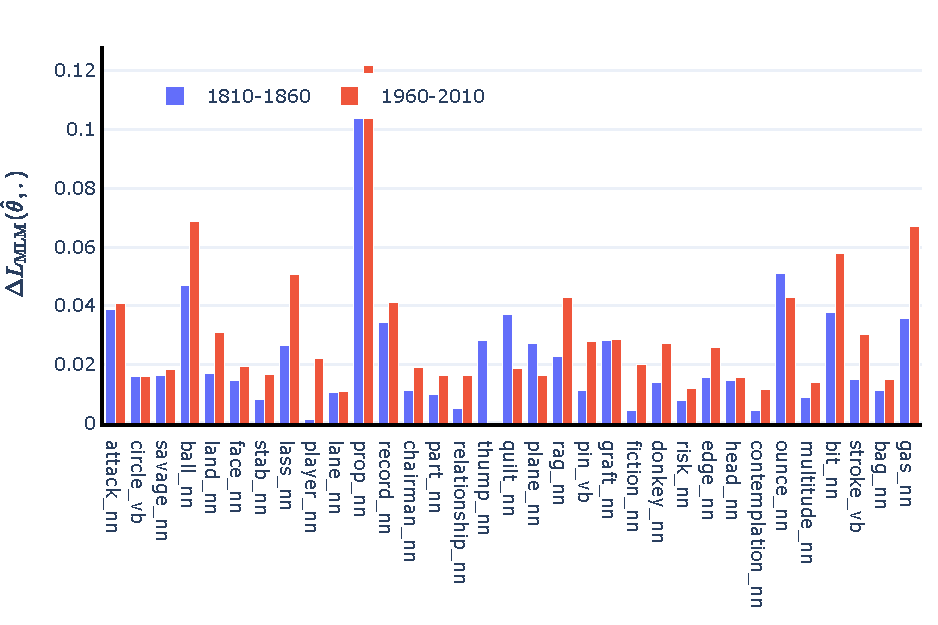
\includegraphics[width=0.8\textwidth]{../project/src/scale_5000-recursion_depth_10000/influences_by_corpus.pdf}
\caption{\textbf{Predicted Influences in different time periods.}}
\label{fig:inf_time}
\end{figure*}

\subsection{Binary Classificaiton}

For binary classification, I achieve 0.7 accuracies, outperforming 20 out of 22 participants in SemEval challenge~\cite{semeval2020}.
Since each team can submit ten trials in the challenge, I try ten different thresholds that equally split the range between maximum influence and min influence and report the best performance.
I show the predicted influences in Fig.~\ref{fig:binary}.
For the words that do not experience any LSC change, the word ``ball'' has the greatest predicted influence. 
From the ground truth rank, the word ``ball'' is the 5th highest word, with a score of $0.409$.
The binary classification considers if the target word gain or loss any sense between two corpora, which is different from how the ground truth of the rank is measured.
%I will discuss the comparison between binary classification and ranking problem in Sec.~\ref{sec:}




\subsection{Ranking}


For the ranking problem, I achieve $0.59$ spearman's correlation, outperforming all 22 participants in SemEval2020~\cite{semeval2020}.
The predicted influences and the ground truth grades are shown in Fig.~\ref{fig:rank}.
One failure case is the word ``plane'', which has a ground truth grade of 0.88, while the predicted influence is as low as 0.02, which ranks middle (19th) in terms of predicted influence.



\begin{figure}[t]
\centering
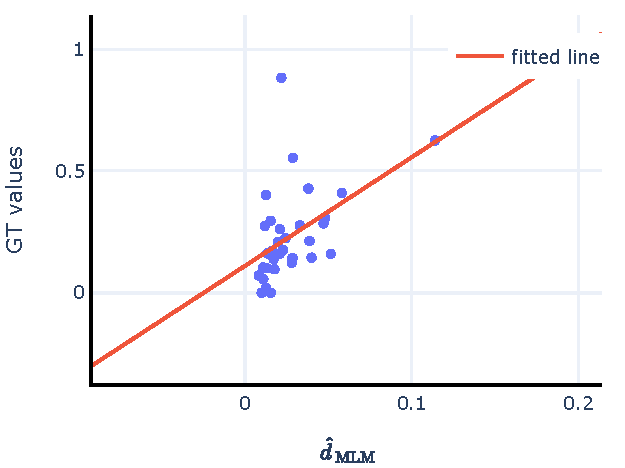
\includegraphics[width=0.5\textwidth]{../project/src/scale_5000-recursion_depth_10000/influences_grade_scatter.pdf}
\caption{\textbf{Predicted Influences vs. ground truth grade.}}
\label{fig:rank}
\end{figure}


\begin{figure*}[t]
\centering
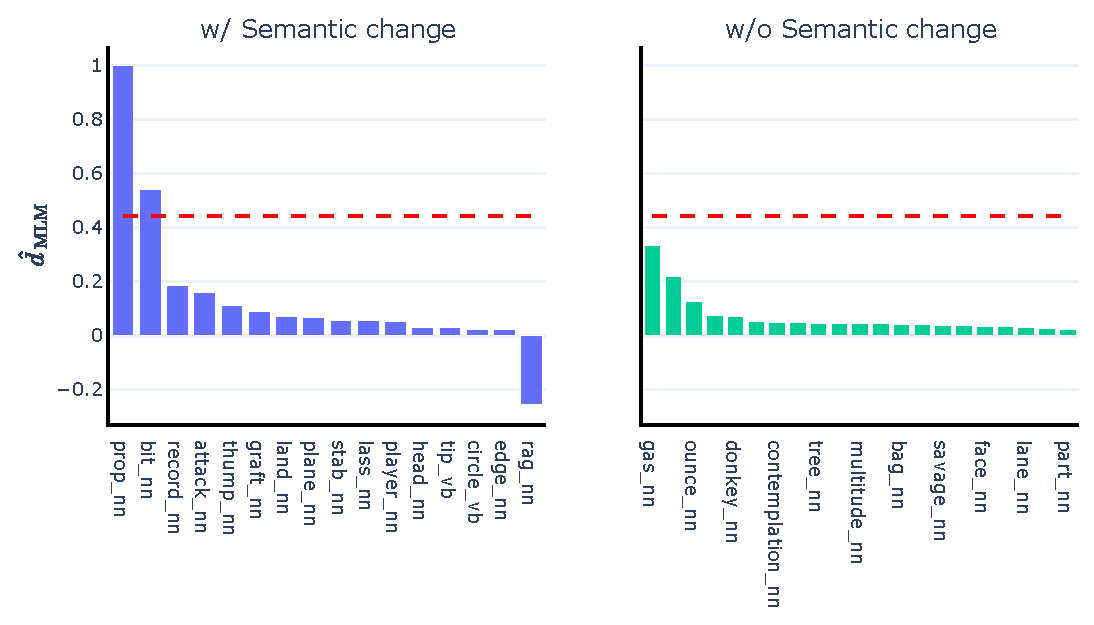
\includegraphics[width=0.8\textwidth]{../project/src/scale_1000-recursion_depth_1000/influences_binary.pdf}
\caption{\textbf{$R_{1000, 1000}$: Predicted Influences in different time periods.} The red dash lines are the threshold for binary classification.}
\label{fig:inf_binary_r_1000_1000}
\end{figure*}


%\subsection{Qualitative Results}

\subsection{Analysis}

\subsubsection{Qualitative Analysis}
The estimated LSC scores are the average predicted influences. 
In Fig.~\ref{fig:inf_time}, I show the predicted influences in $C_1$ and $C_2$. 
The word ``player'', ``fiction'', and ``relationship'' have the most difference between predicted influences in $C_1$ and $C_2$, more than 300\%.
For certain words, the computation of inverse HVP diverges. In these cases, I treat them as an outlier and do not consider their values.


\subsubsection{Hyperparameter Analysis}
To compute the influence functions, we adopt the approximation approach~\cite{second-order-approx}, which includes several hyperparameters.
When performing the approximation, two hyperparameters govern the stability of the approximation, scale and recursion depth. 
As mentioned in Sec.~\ref{sec:impl_details}, we set them to be $(5000, 10000)$, denoted as $R_{5000, 10000}$.
In this section, we show other two configurations $R_{1000, 1000}$ and $R_{1000, 10000}$.
The comparison of three different configurations in binary classification and the ranking problem is shown in Table.~\ref{tab:hyperparams}.
Both the performances of binary classification and the ranking problem vary a lot.
The binary classification results in $R_{1000, 1000}$ might look nice, achieving 62\% accuracy, outperforming 14 out of 22 teams in the SemEval2020 challenges.
However, from Fig.~\ref{fig:inf_binary_r_1000_1000} and Fig.~\ref{fig:inf_scatter_r_1000_1000}, there are only two positive predictions and all the other are predicted negative. 

From the hyperparameters analysis results, the proposed approach requires lots of tuning to get great results.


\begin{table}[t]
\centering
\resizebox{\linewidth}{!}{%
\begin{tabular}{@{}rcc@{}}
\toprule
 & \multicolumn{1}{r}{Binary Classification} & \multicolumn{1}{r}{Ranking Problem} \\ \midrule
\multicolumn{1}{r|}{$R_{5000, 10000}$} & \textbf{0.7} & \textbf{0.59} \\
\multicolumn{1}{r|}{$R_{1000, 10000}$} & 0.37 & 0.57 \\
\multicolumn{1}{r|}{$R_{1000, 1000}$} & 0.62 & 0.27 \\ \bottomrule
\end{tabular}%
}
\caption{\textbf{Comparison between different hyperparameters configurations.}}
\label{tab:hyperparams}
\end{table}





\begin{figure}[t]
\centering
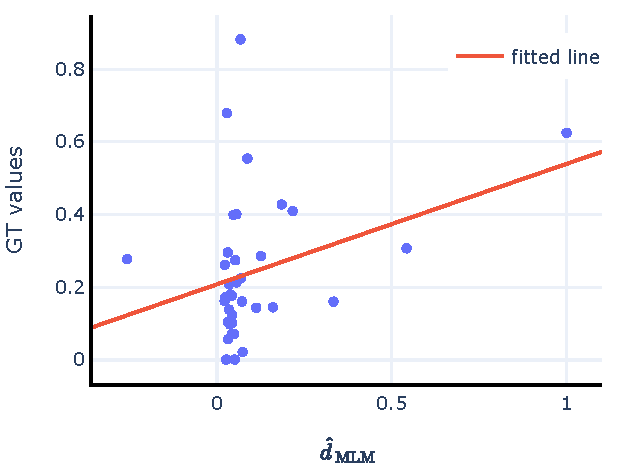
\includegraphics[width=0.5\textwidth]{../project/src/scale_1000-recursion_depth_1000/influences_grade_scatter.pdf}
\caption{\textbf{$R_{1000, 1000}$: Predicted Influences vs. ground truth grade.}}
\label{fig:inf_scatter_r_1000_1000}
\end{figure}
\section{Discussion}

The proposed approach shows that the influences function is highly correlated with LCS, achieving 0.7 in binary classification and 0.59 in spearman's correlation in the ranking problem.
However, the estimation of the influence function is time-consuming and not stable.
For each term in Eq.~\ref{eq:influence_fn_mlm}, it takes more than 20 minuites to compute.
The bottleneck is the approximation of inverse HVP. 
The approximation is done recursively, so it's not parallelizable. In our case, it takes 10000 recursion steps to reach convergence.
Additionally, the computation is not stable for some words (e.g., ``trump''), leading to divergence.
The computational expensive and instability hamper it from performing LCS in a continuous fashion. For example, monitoring the LCS for an extended period will be prohibitively computationally expensive.



% Entries for the entire Anthology, followed by custom entries
\bibliography{anthology,custom}

%\appendix

%\section{Example Appendix}
%\label{sec:appendix}

%This is an appendix.

\end{document}
